\documentclass[twoside, 12pt]{article}
\usepackage[
  a4paper,
  inner=3.5cm,
  outer=2.5cm,
  bmargin=2.5cm,
  tmargin=2.5cm
]{geometry}

% \usepackage[
%   a4paper,
%   bmargin=2.5cm,
%   tmargin=2.5cm,
%   rmargin=2.5cm,
%   lmargin=3.5cm
% ]{geometry}

\usepackage[utf8]{inputenc}
\usepackage{lmodern}
\usepackage[T1]{fontenc}
\usepackage[hungarian]{babel}

\usepackage{array}
\usepackage{makecell}

\usepackage{graphicx}
\graphicspath{ {../images/} }

\usepackage[letterspace=150]{microtype}
\usepackage{setspace}

\usepackage{pdfpages}
\usepackage{float}

\usepackage{tikz}
\newcommand*\circled[1]{
  \tikz[baseline=(char.base)]{
    \node[shape=circle,draw,inner sep=1pt] (char) {#1};
  }
}

% \onehalfspacing
\linespread{1.25}
\begin{document}

\begin{titlepage}
  \setlength{\tabcolsep}{0pt}

  \noindent\begin{tabular}{m{4cm} m{8cm}}
    \makecell{
      
\includegraphics[width=3cm]{elte_cimer_szines.jpg}
    }
    &
    \textbf{\textls{\makecell{
      Eötvös Loránd Tudományegyetem \\
      Informatikai Kar \\
      Média- és Oktatásinformatika Tanszék
    }}} \\
  \end{tabular}

  \begin{center}
    \rule{14cm}{1pt}\hfill
  \end{center}

  \vspace{3cm}

  \begin{center}
    \LARGE{\textbf{
      Földi monitorozó és vezérlési kezelőfelület önrepülő drónokhoz
    }}
  \end{center}

  \vspace{3cm}

  \begin{center}
    \noindent\begin{tabular}{m{7cm} m{7cm}}
      \makecell{
        Dr. Horváth Győző \\
        Belső témavezető \\
        Média- és Oktatásinformatika Tanszék \\
        Egyetemi adjunktus
      }
      &
      % \makecell{

      % }
      \\[3cm]
      \makecell{
        Dr. Nepusz Tamás \\
        Külső témavezető \\
        CollMot Robotics Ltd. \\
        Informatikai vezető
      }
      &
      \makecell{
        Donkó István \\
        Szerző \\
        ELTE IK \\
        Programtervező Informatikus BSc hallgató
      }
      \\
    \end{tabular}

    \vfill

    \large{2018, Budapest}
  \end{center}
  \thispagestyle{empty}
\end{titlepage}

% \noindent\hfill\rule{14cm}{1pt}\hfill
% \noindent\makebox[\linewidth]{\rule{\paperwidth}{0.4pt}}
% \noindent\rule{\textwidth}{1pt}


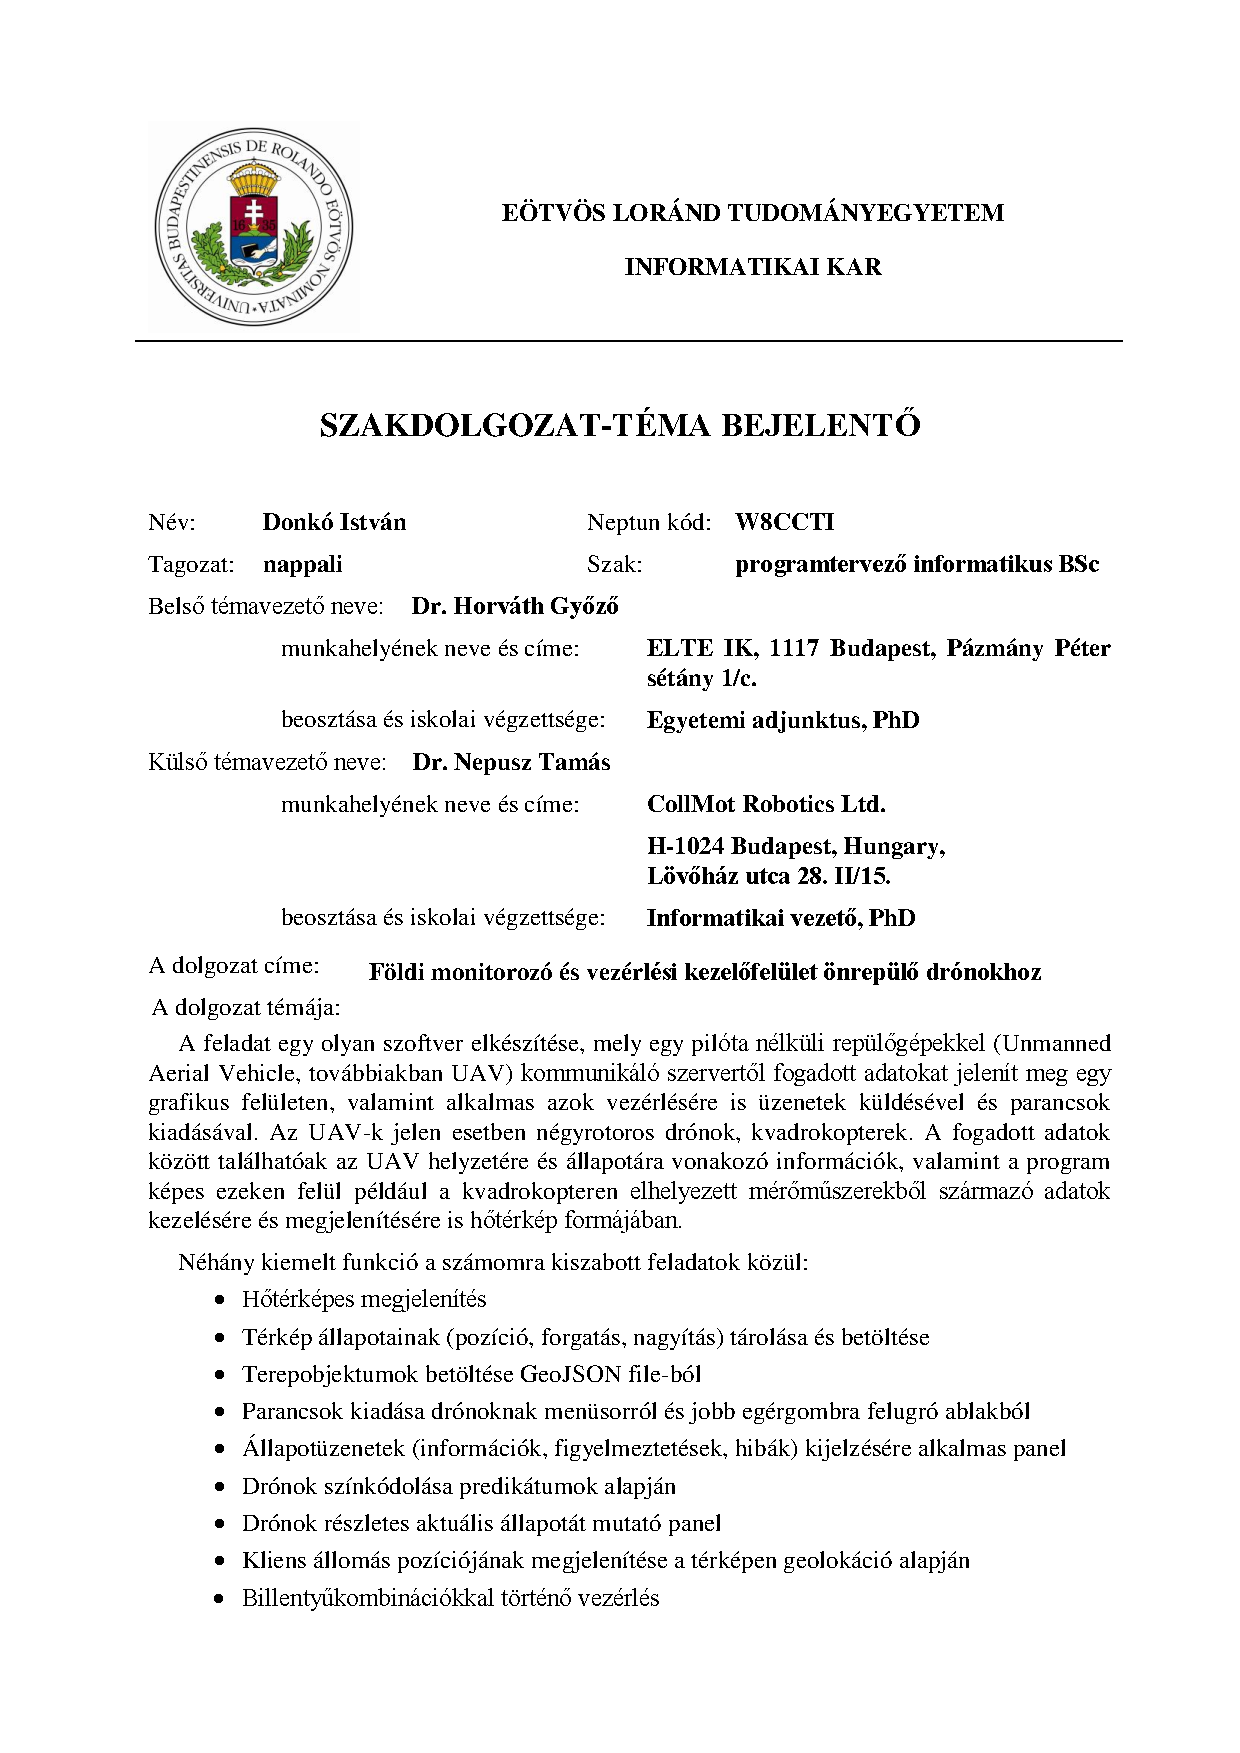
\includepdf[pages={-}]{../Donko_Istvan_W8CCTI_PTI_Bsc_temabejelento_lap_szakdolgozat_final.pdf}

\tableofcontents\newpage

\part{Bevezetés}

\section{Bevezetés}

Napjainkban egyre inkább terjednek el a különféle drónok, távirányítással vagy
akár önálló módon repülő többrotoros kopterek formájában. Számos nagyobb gyártó
(például DJI, Parrot) is kínál a fogyasztói piacon készen megvásárolható
termékeket, továbbá számtalan lelkes ember áll neki otthon kísérletezni ilyesmi
szerkezetek építésével.

Az ELTE Biológiai Fizika Tanszékével szoros együttműködésben a CollMot kft.
rendelkezik körülbelül 40 saját építésű kopterrel, amelyeken az alacsonyabb
szintű motorvezérlő pilótaprogram felett belső fejlesztésű rendszerük fut.

A szóban forgó drónok felhasználása igencsak változatos. Kutatási oldalról
például különböző tudományos szimulációk tesztelésére is alkalmasak, mint
akár madarak vagy halak viselkedésének vizsgálata egyszerű fizikai törvényeken
alapuló rajzási modellek evolúciójának segítségével. Ezen felül szolgálhatnak
továbbá látványelemként is egy előre betáplált koreográfia útvonalának
végigrepülése közben LED lámpájuk fényerejét és színét változtatva.

\begin{figure}[h!]
  \center
  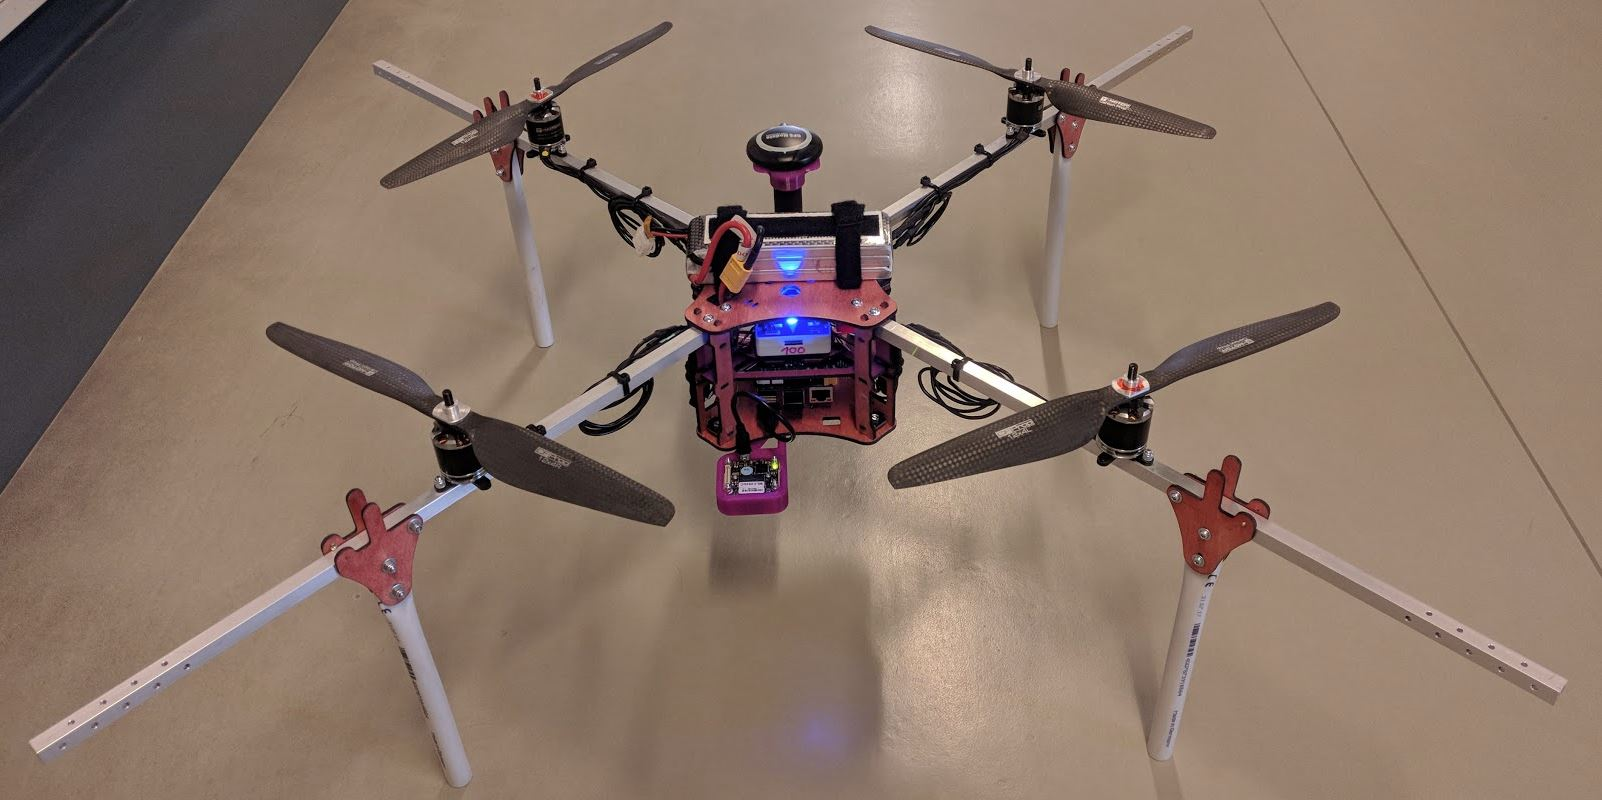
\includegraphics[width=0.8\textwidth]{drone.jpg}
  \caption{Fénykép a fent említett kopterek egy példányáról}
  \label{fig:drone}
\end{figure}

A FlockWave szoftver ötlete az ezen drónok monitorozására és vezérlésére készült
régebbi GroundControl nevű parancssori eszköz (lásd \ref{fig:groundcontrol}.
ábra) grafikus megjelenítéssel rendelkező megoldásra történő leváltásának
céljával fogalmazódott meg.

% TODO: Két mondatba?

Léteznek már kész, elérhető szoftverek hasonló célokra, azonban a kereskedelmi
drónokhoz való, gyártók által mellékelt programok általában nem flották, hanem
leginkább csak egy-egy drón kezelésére alkalmasak, ráadásul zártak, tehát csak
a gyártó saját termékeivel működnek.

Természetesen nem új gondolat a több kopter kezelésére is képes általános
vezérlési felület sem. Ilyen az UgCS nevű program (https://www.ugcs.com), amely
számos protokollt támogat, így sok gyártó eszközeivel képes kommunikálni,
ráadásul elméletileg korlátlan számú drónt tud kezelni, azonban zárt, és így a
piacon lévő egyeduralmának köszönhetően nagyon drága.

Nyílt forráskódú kezdeményezés említésének céljából érdemes a QGroundControl-t
(http://qgroundcontrol.com/) kiemelni, ami egy nagyon sokoldalú program,
azonban sajnos egyidejűleg csak egy kopter kezelésére képes.

\begin{figure}[H]
  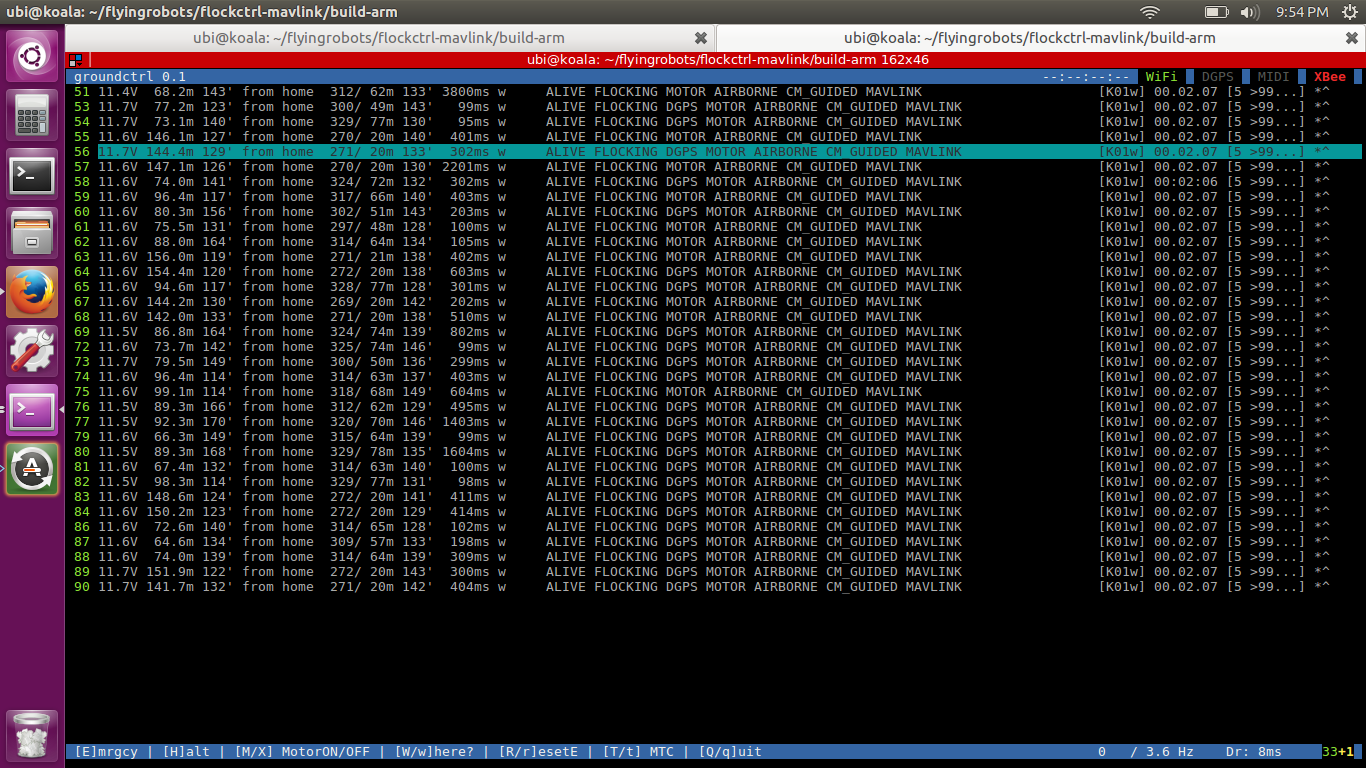
\includegraphics[width=\textwidth]{groundcontrol.png}
  \caption{Képernyőfotó a lecserélésre szánt régi karakteres kezelőfelületről}
  \label{fig:groundcontrol}
\end{figure}

\noindent A FlockWave szoftver ötletének a megvalósítási folyamatába
kapcsolódtam be még abban a kezdeti szakaszban, amikor a program körülbelül csak
a drónok pozícióját tartalmazó szerverről érkező csomagok feldolgozására és az
ezekből származó adatok alapján történő térképen való megjelenítésére volt
alkalmas. Ekkor lett a feladatom a rendszer további funkciókkal történő
ellátása. Ezek közül néhányat mutatok be kiemelve ebben a szakdolgozatban.


\part{Felhasználói dokumentáció}

\section{Követelmények}

Szerver oldalon tehát szükséges egy számítógép, amely hardware tekintetében
rendelkezik Wi-Fi rádióval, vagy csatlakoztatva van hozzá XBee adó-vevő.
Szoftver területén megfelelő Wi-Fi vagy XBee driver, illetve a szerver
kódjának futtatásához \verb|python 3.6| a követelmény.

A kliens oldal kódjának lefordítása \verb|nodejs| által zajlik, a függőségek
kezelését az \verb|npm| csomagkezelő végzi, az elkészült állomány egy
webszerverről kiszolgálva egy böngészőből érhető el, vagy pedig \verb|electron|
segítségével becsomagolva önállóan futtatható programként.

A forráskód birtokában annak gyökérmappájában kiadva az \verb|"npm install"|
parancsot telepíthetőek a függőségek. Ezt követően az \verb|"npm start"|
utasítás elvégzi a JavaScript kód kötegelését és kiszolgálja a kliens
alkalmazást alkotó tartalmakat egy webszerver segítségével, amely egy
böngészőből alapértelmezetten a http://localhost:8080/ címen érhető el.

A program önállóan futó alkalmazásként történő használatának előfeltétele, hogy
az electron csomag globálisan telepítve legyen. Amennyiben ez teljesül, akkor az
\verb|"npm run start:electron"| parancs indítja el saját külön ablakban a
klienst. A terjesztésre szánt futtatható állomány előállításához szükség van még
ezeken felül az \verb|"electron-builder"| meglétére. Ennek a hordozható file-nak
a létrehozását az \verb|"npm run dist"| utasítás kiadásával lehet kezdeményezni.

% TODO
(Legyen rajta a DVD-n a node\_modules mappa?)

\section{Áttekintés}

A rendszer működéséhez szükséges egy szerver, ami Wi-Fi vagy XBee alapú rádiós
kommunikáció segítségével fogadja az adatokat a drónoktól, valamit továbbítja
feléjük a kiadott parancsokat. Ehhez a szerver a felhasználói kliens WebSocket
protokoll segítségével csatlakozhat. A kliens program futtatható oly módon, hogy
egy központi webszerver egy helyi hálózaton kiszolgálja a FlockWave kliens
alkalmazás webes tartalmát (csomagolt JavaScript, stíluslapok, képek, stb.), így
ez tetszőleges olyan eszközről elérhető, amely rendekezik (lehetőség szerint
Google Chrome) böngészővel, illetve Windows, Linux és MacOS (OSX) rendszerekre
elérhető Electron segítségével becsomagolt önműködő állomány is.

\begin{figure}[H]
  \centering
    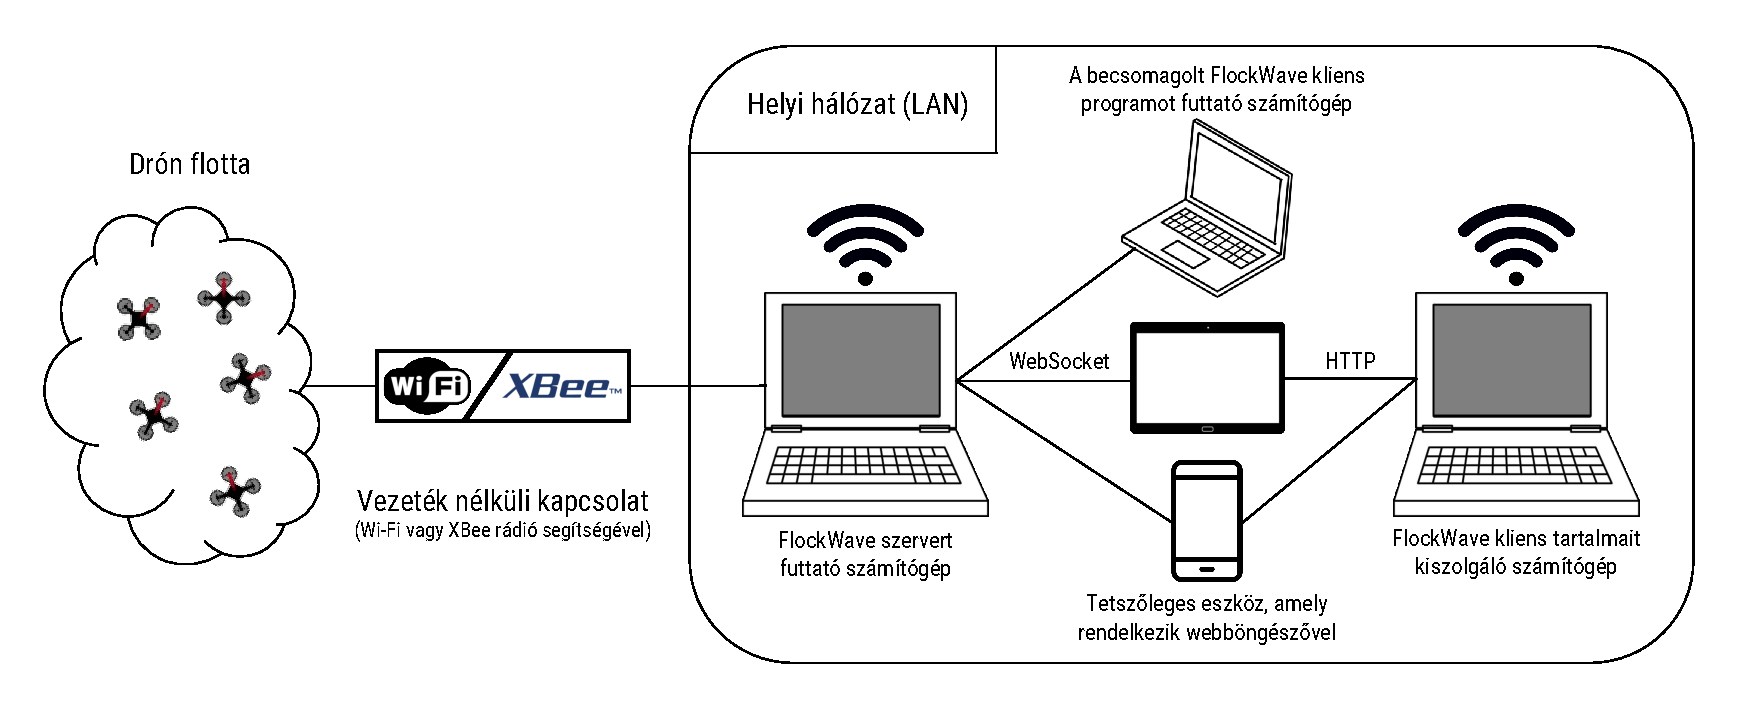
\includegraphics[width=\textwidth]{operational_structure_2.pdf}
  \caption{A rendszer felépítése}
\end{figure}

\textit{Megjegyzés: Természetesen semmi sem zárja ki, hogy a FlockWave szerver
futtatását és a kliens tartalmának kiszolgálását ugyanaz a számítógép végezze.}

\section{A felület elérése}

A kliens oldali program két különböző módon is elérhető a felhasználók számára:
\begin{itemize}
  \item Tetszőleges internetböngészővel rendelkező eszközről a helyi hálózaton
  futó szerver segítségével. Ekkor a böngésző címsorába beírva a szerver címét
  egyből a FlockWave kliens felületét kapjuk, ami egy SPA (Single Page
  Application), tehát összesen egy lapból áll, nem alkalmaz navigációt.
  \item Windows, Linux vagy MacOS (OSX) rendszerek alatt Electron segítségével
  becsomagolt állománnyal rendelkező önálló alkalmazásként.
\end{itemize}

A felület megnyitása után szükséges csatlakozni a drónokkal történő közvetlen
kommunikációt végző FlockWave szerver alkalmazást futtató számítógéphez. Ez
lehetséges az elérési cím és port (alapértelmezetten 5000) manuális megadásával,
illetve az SSDP (Simple Service Discovery Protocol) hálózati felderítési
protokoll segítségével.



\section{A felület kezelése}

\subsection{Kezdeti állapot}

Alapállapotban a felület a térképet jeleníti meg, mellette pedig az eltárolt
pozíciók kezelésére alkalmas panelt, valamint az ismert drónok listáját. További
felületi elemek érhetőek el a fülekre kattintva, illetve a bal oldalon található
sávról ( \ref{fig:initial_state}. ábra /\circled{1}) kattintással vagy húzással
a felületre helyezve.

\begin{figure}[H]
  \center
  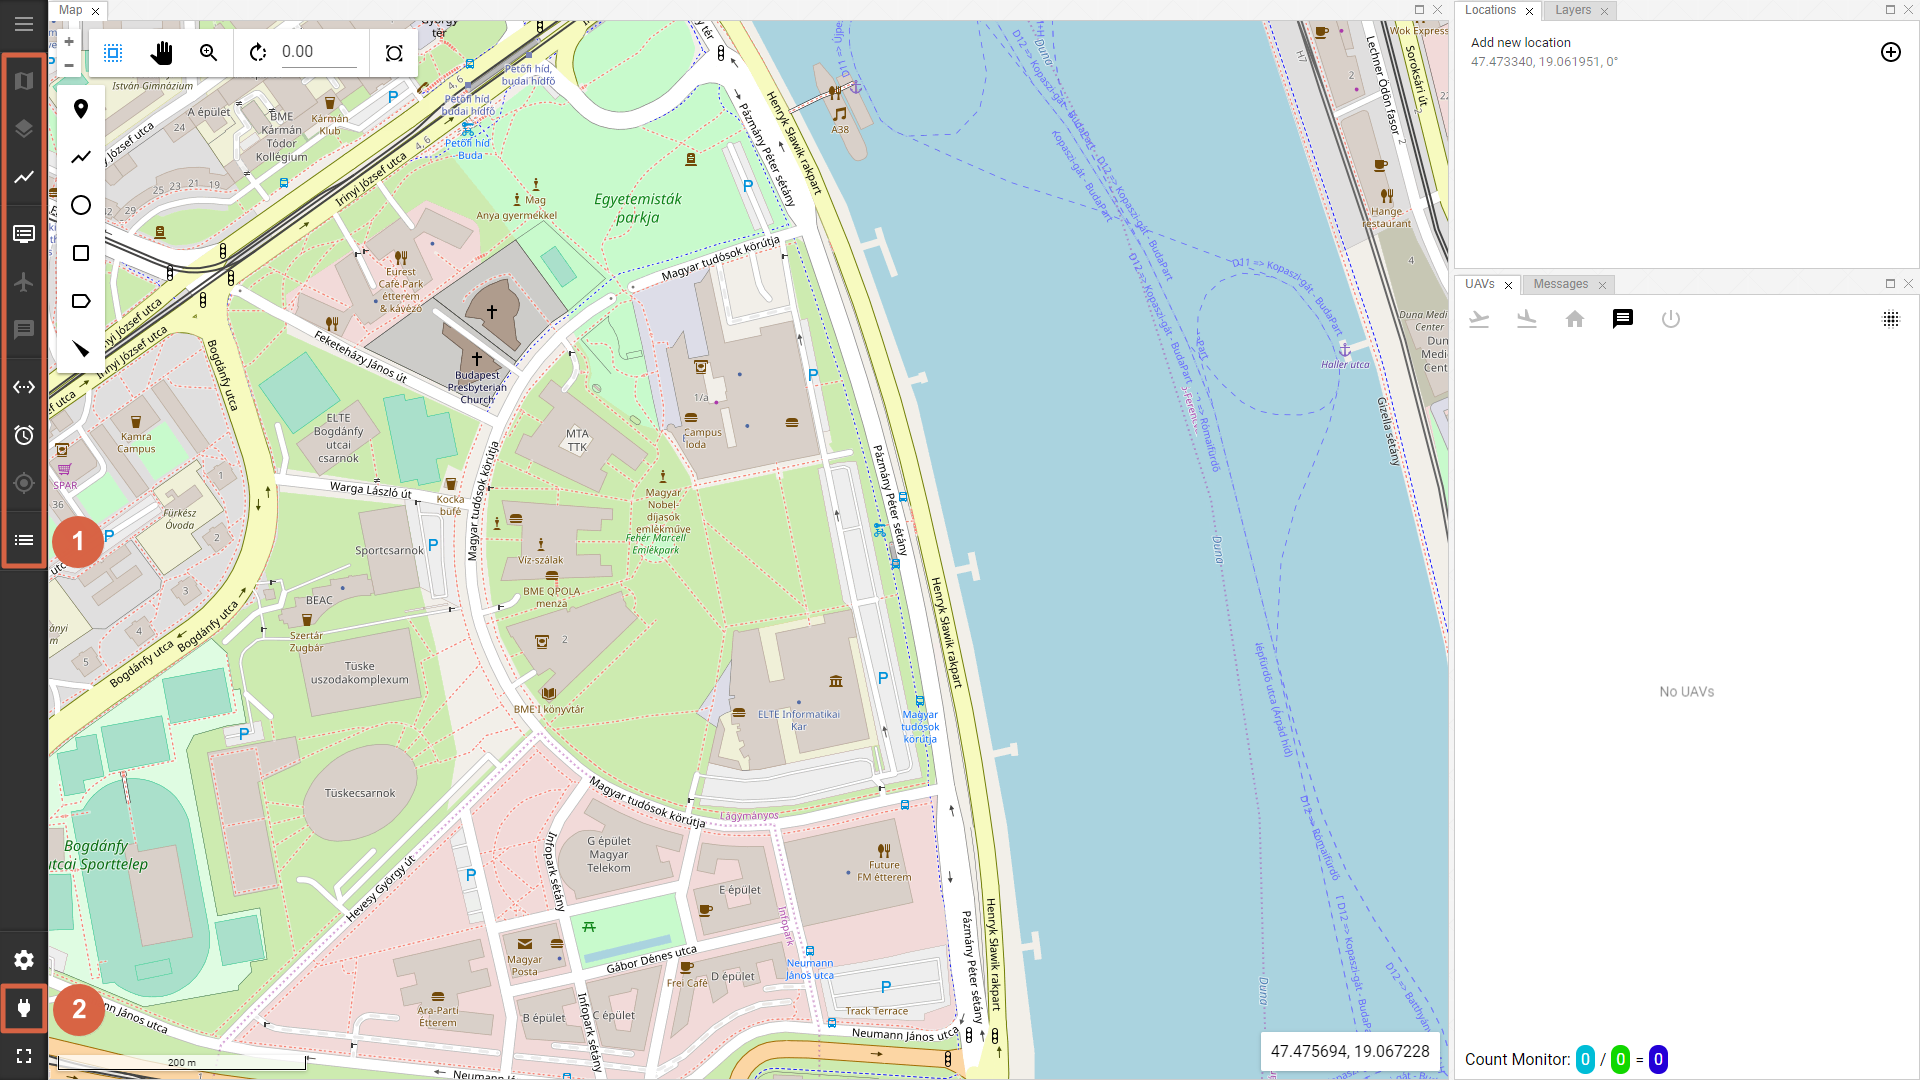
\includegraphics[width=\textwidth]{screenshots/initial_state.png}
  \caption{A kliens program alapállapota}
  \label{fig:initial_state}
\end{figure}


\subsection{Csatlakozás a szerverhez}

A szerverhez való csatlakozásához meg kell adni annak elérési adatait. Ezt a
\ref{fig:initial_state}. ábra /\circled{2} jelölésű gombján történő kattintás
után megjelenő dialógusablakban tehetjük meg.

\begin{figure}[H]
  \center
  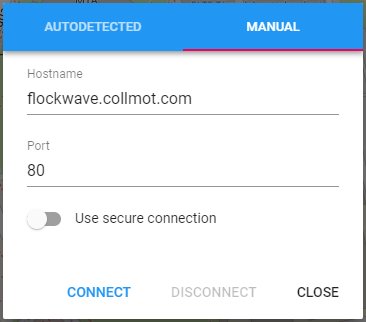
\includegraphics[width=0.5\textwidth]{screenshots/connection_dialog.png}
  \caption{A szerverhez való csatlakozásra szolgáló dialógusablak}
  \label{fig:connection_dialog}
\end{figure}

Sikeres csatlakozás esetén a dialógusablak megnyitására szolgáló gomb mellett
megjelenik egy kis zöld színű teli kör alakú jelölő, az UAVs című panelben és a
térképen pedig láthatóvá válnak a szerverrel aktuálisan kapcsolatban álló
drónok.


\subsection{Hőtérképes megjelenítés}

Hőtérképes megjelenítés segítségével a drónokon elhelyezett műszerek mérései
ábrázolhatóak vizuális módon. Ehhez először egy hőtérkép típusú réteg
létrehozása szükséges a rétegek panelen az "Add new layer", majd pedig azon
belül a "Heatmap" opciót választva.

Ekkor a rendszer lehetőséget biztosít a megfigyelni kívánt csatornákra történő
fel-- és leiratkozásra. Ez az "Edit subscriptions" gomb által megjeleníthető
dialógusablakban tehető meg. Ezen feliratkozások adott drónokon (UAV) elérhető
eszközök (device) csatonáira (channel) vonatkoznak.

Beállítható továbbá egy küszöbszint, ami alatt az értékeket fehérrel jelzi,
valamint a színskála két széléhez tartozó érték is megadható manuálisan, vagy
pedig bekapcsolható az automatikus skálázás, amely esetén minden beérkező érték
feldolgozásakor frissíti a határokat a rendszer, amennyiben ez szükséges.
Személyre szabhatóak a színskála végpontjainak színárnyalatai, valamint a
színezési függvény is kiválasztható. (Lineáris vagy logaritmikus.)

Ezen felül megadható a mérési pontok közötti minimális távolság, bekapcsolható a
rácspontokhoz történő igazítás, továbbá törölni lehet az eddig mért adatokat.

A kép (\ref{fig:heatmap}. ábra) például egy logaritmikus színezésű, 5 méteres
sűrűségű rácspontokra igazított hőtérkép látható, amely egy szimulált pontszerű
forrásból származó radioaktív mérés eredményeit ábrázolja.

\begin{figure}[H]
  \center
  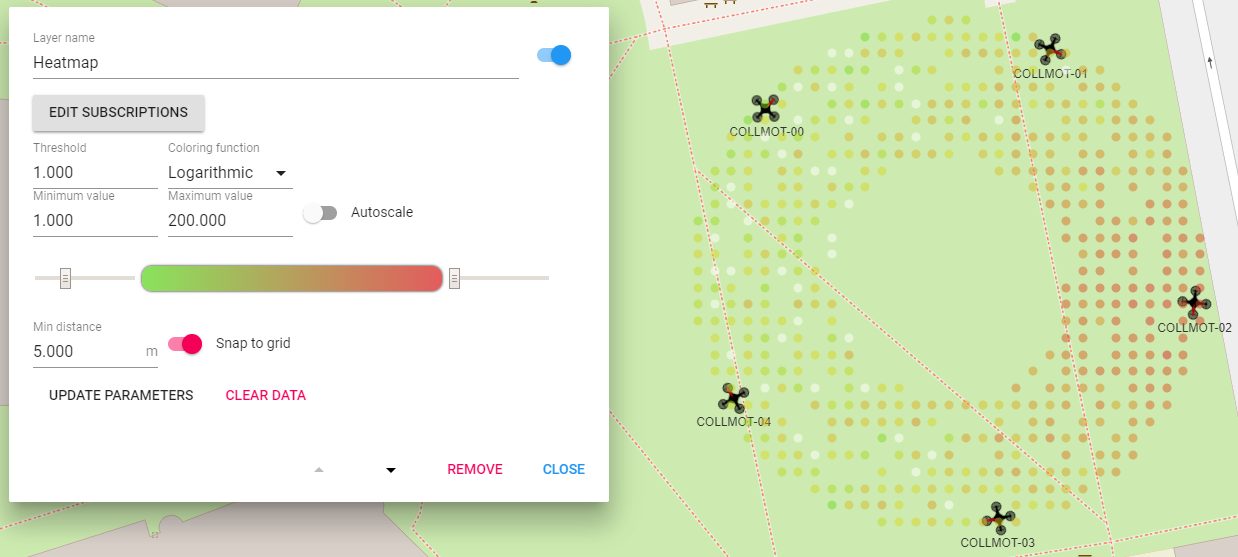
\includegraphics[width=\textwidth]{screenshots/heatmap.png}
  \caption{Egy hőtérkép kinézete}
  \label{fig:heatmap}
\end{figure}


\subsection{Térkép állapotainak elmentése és betöltése}

Az alkalmazás lehetőséget biztosít adott térkép állások (középpont, nagyítás és
elforgatás) tárolására későbbi betöltés céljából. Ehhez felületi elemként
elérhető a kép (\ref{fig:saved_locations}. ábra) bal oldalán látható listát
tartalmazó panel, mely az eddig elmentett opciókat tartalmazza. Egy elemre
rákattintva betölthető az adott állapot, ekkor a térkép animálva átvált egy,
az eltárolt középponttal, nagyítással és elforgatással rendelkező nézetre. A
listaelemek mellett szereplő fogaskerék ikon pedig a kép jobb oldalán látható
dialógusablakban nyitja meg szerkesztésre a kiválasztott helyet. Itt törölhető
is az adott bejegyzés, ha már nincs rá szükség.

Új hely az első elemre ("Add new location") kattintva adható hozzá a
listához. Ekkor a dialógusablak a térkép aktuális állapotának értékeivel
kitöltve nyílik meg, így az könnyen elmenthető, vagy pedig kézzel bevihetőek
kívánt adatok.

\begin{figure}[H]
  \center
  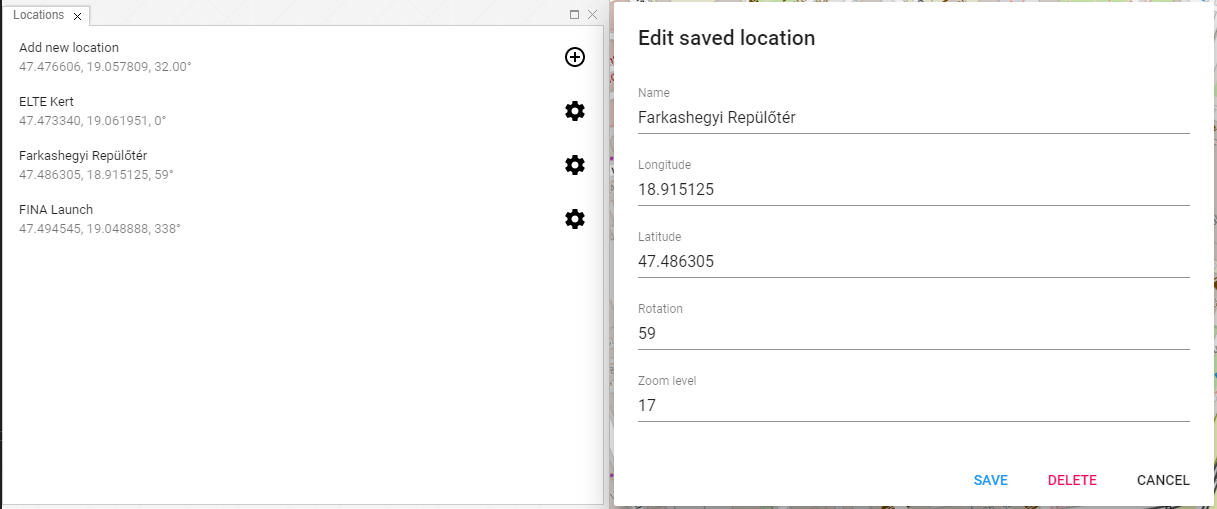
\includegraphics[width=\textwidth]{screenshots/saved_locations.png}
  \caption{A mentett pozíciók panelje és a szerkesztésükre alkalmas dialógusablak}
  \label{fig:saved_locations}
\end{figure}


\subsection{GeoJSON megjelenítése}

A GeoJSON egy elterjedt térképészeti formátum, mely geográfiai objektumok
leírására alkalmas. A jelenlegi legfrissebb (2016-ban kiadott) pontos
specifikációja elérhető itt: https://tools.ietf.org/html/rfc7946

Drónok vezérlésénél és monitorozásánál szükség lehet előre megadott létező vagy
virtuális terepobjektumok megjelenítésére a térképen, mint például környező
akadályok, épületek, vagy esetleg egy kijelölt repülési zóna.

Ezek megjelenítéséhez egy speciális réteg hozzáadása szükséges. Ez a rétegek
panelen az "Add new layer" gomb megnyomásával lehetséges. Amennyiben az ezt
követően felugró dialógusablakban a GeoJSON opció kerül kiválasztásra, akkor az
alkalmazás felkínálja a réteg beállításait. Megadhatóak a megjeleníteni kívánt
GeoJSON objektum kirajzolásához felhasználandó színek külön a körvonalhoz,
valamint a kitöltéshez, továbbá testreszabható a körvonal vastagsága. A GeoJSON
forrásszöveg elhelyezése is a dialógusablakban lévő szövegdobozban történik,
majd pedig az "IMPORT GEOJSON" gombot megnyomva a forrás által meghatározott
objektum megjelenik a térképen.

GeoJSON formátumú adatok előállításához több különböző szoftver is elérhető, de
akár saját kézzel is elkészíthető az objektumokat leíró forráskód. Az alábbi
illusztráción (\ref{fig:geojson}. ábra) elhelyezett poligon például a
http://geojson.io címen elérhető szerkesztő segítségével készült.

\begin{figure}[H]
  \center
  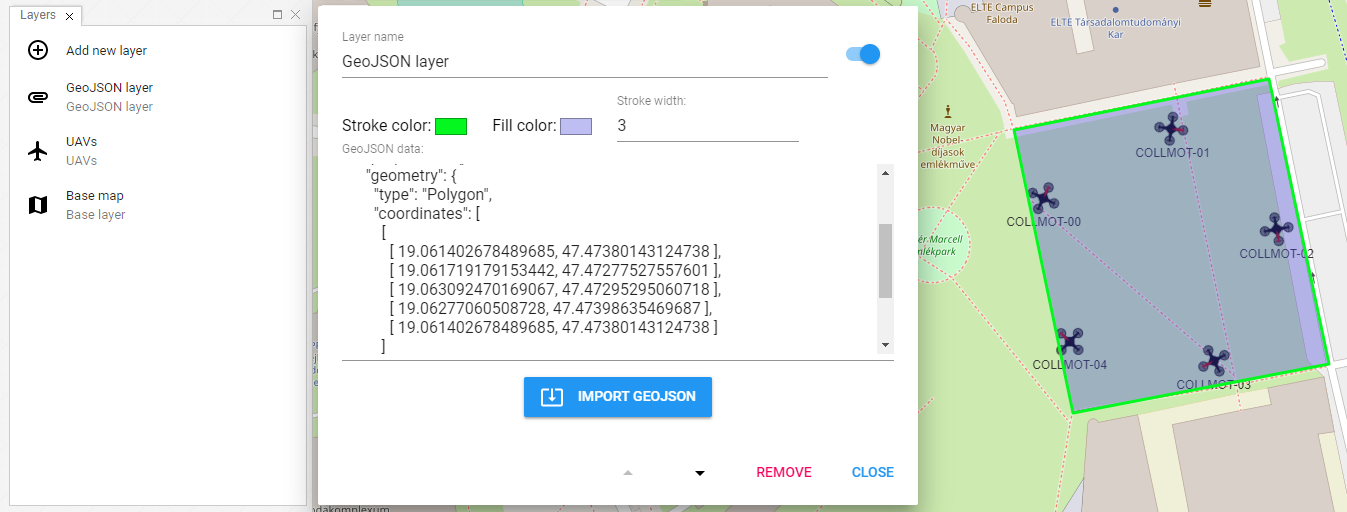
\includegraphics[width=\textwidth]{screenshots/geojson.png}
  \caption{Egy poligont megjelenítő GeoJSON réteg}
  \label{fig:geojson}
\end{figure}

\subsection{Parancsok kiadása drónoknak}

A drónoknak jelenleg négy fajta parancs adható ki: felszállás, leszállás,
visszatérés a kiindulópontra valamint kikapcsolás. Ezek a lehetőségek elérhetők
a térképen történő jobb egérgombbal végzett kattintáskor felugró menüből
( \ref{fig:commands}. ábra /\circled{1}), valamint a drónok listáját tartalmazó
panel tetején található eszköztárról ( \ref{fig:commands}. ábra /\circled{2}).
Egy parancs kiadását követően a szerver visszajelzést küld annak végrehajtásának
sikerességéről, ez a válasz pedig bekerül bejegyzésként az eseménynaplóba.

\begin{figure}[H]
  \center
  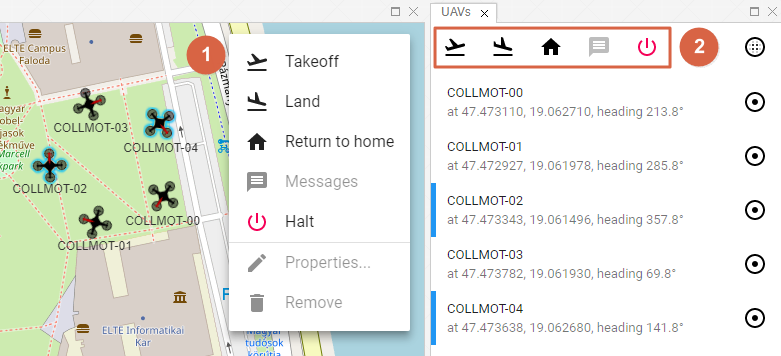
\includegraphics[width=\textwidth]{screenshots/commands.png}
  \caption{A drónoknak történő parancskiadás módjai}
  \label{fig:commands}
\end{figure}


\subsection{Állapotüzenetek kijelzésére alkalmas panel}

A rendszer naplóbejegyzéseit megjelenítő panel alapbeállításként nincs
bekapcsolva, a bal oldali sávról érhető el. A felületre helyezve egy szűrhető
és rendezhető táblázat formájában jeleníti meg az állapotüzenetek listáját.
Alapértelmezetten az üzenetek érkezésének időpontja szerint van csökkenő
sorrendbe rendezve, azonban ez átállítható például az üzenetek szintjei szerinti
rendezésre, továbbá szűrések alkalmazhatók bármelyik oszlopon.

\textit{
  Bővebben a szűrhető és rendezhető táblákról lásd:
  \ref{filterable_sortable_table}
}

\begin{figure}[H]
  \center
  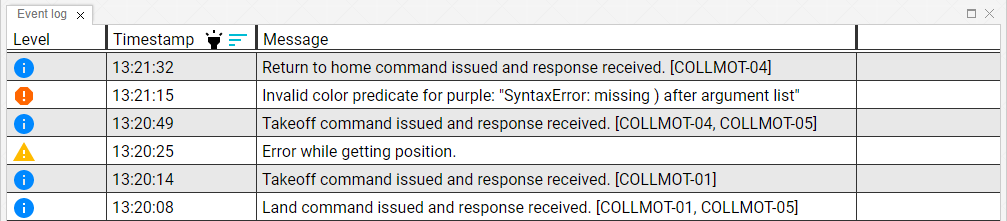
\includegraphics[width=\textwidth]{screenshots/log.png}
  \caption{Példa az állapotüzeneteket tartalmazó lista megjelenésére}
  \label{fig:log}
\end{figure}


\subsection{Drónok színkódolása predikátumok alapján}

A drónok színkódolására vonatkozó predikátumok megadására a kopter piktogramok
megjelenítéséért felelős réteg (UAVs) beállításai között van lehetőség.
Hat szín áll rendelkezésre, ezekhez egy egy JavaScript függvénytörzs rendelhető
hozzá. Az "Apply changes" gomb megnyomásakor a rendszer megvizsgálja a mezők
értékét, és amelyikben hibát talál, azt megjelöli, valamint bejegyzést készít az
eseménynaplóba a hiba pontos szövegéről, a többit pedig elmenti és alkalmazza a
drónokra oly módon, hogy a drónok azonosítóit egyesével paraméterül adja
függvényeknek, és olyan színűre színezi az adott piktogramot, amelyik színhez
tartozó függvény igazra értékelődött ki.

Az alábbi példában (\ref{fig:uav_coloring}. ábra) a lila színhez tartozó
predikátum hibás, a kettőnél kisebb számra végződő azonosítóval rendelkező
koptereket zöldre, a négynél nagyobbakat narancssárgára, a "COLLMOT-02"-es és
"COLLMOT-04"-es drónt pedig kékre színeztük.

\begin{figure}[H]
  \center
  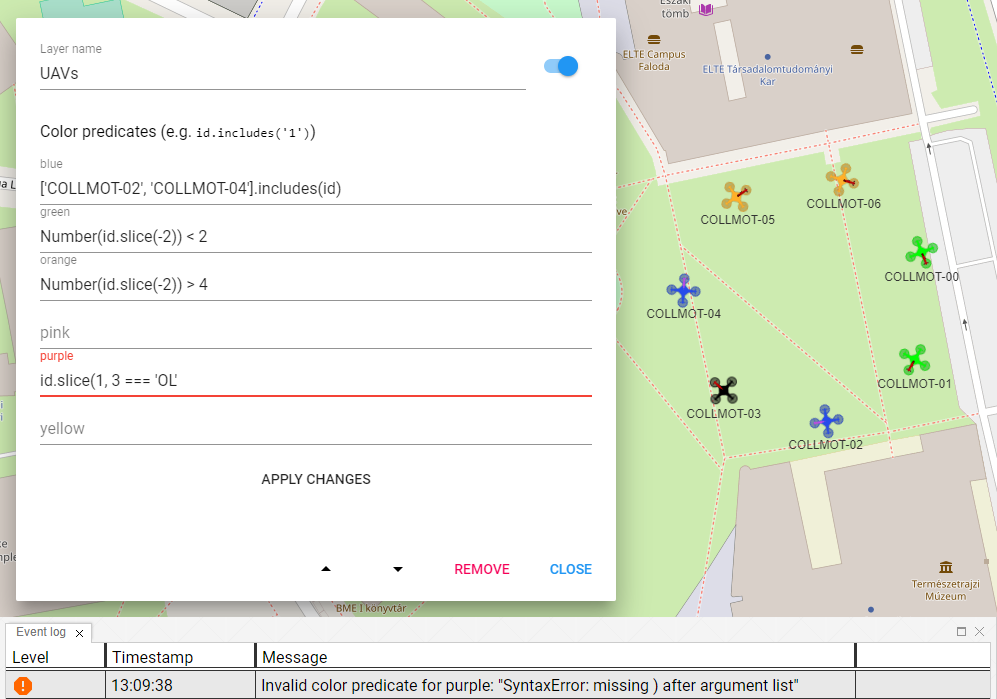
\includegraphics[width=\textwidth]{screenshots/uav_coloring.png}
  \caption{Példa néhány predikátumra}
  \label{fig:uav_coloring}
\end{figure}

\subsection{Drónok részletes aktuális állapotát mutató panel}

A régi karakteres felület előnyének fenntartására, az elérhető információ tömör
formában történő megtekintésére szolgáló "Ground Control View" nézet
alapbeállításként rejtve van, a bal oldali sávról aktiválható. Ekkor egy
szűrhető és rendezhető táblázatként válnak benne elérhetővé a drónok aktuális
adatai.
A név oszlop szöveg típusú szűréssel és rendezéssel rendelkezik, az összes többi
intervallum típusú, így könnyen megkereshetőek például egy adott kritikus
akkufeszültség alatt lévő drónok, vagy mondjuk lehet rendezni őket az
elhelyezkedésük alapján a szélességi és hosszúsági koordinátáik szerint.

\textit{
  Bővebben a szűrhető és rendezhető táblákról lásd:
  \ref{filterable_sortable_table}
}

\begin{figure}[H]
  \center
  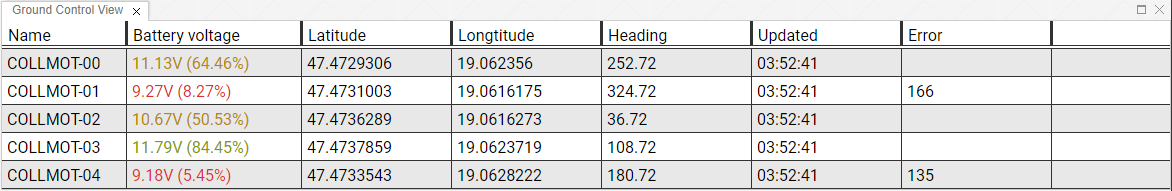
\includegraphics[width=\textwidth]{screenshots/ground_control_view.png}
  \caption{A drónok adatai egy szűrhető és rendezhető táblázatban}
  \label{fig:ground_control_view}
\end{figure}

\subsection{Kliens állomás pozíciójának megjelenítése geolokáció alapján}

Amennyiben a kliens alkalmazást futtató eszköz rendelkezik geolokáció
megállapítására alkalmas szolgáltatással, akkor az "Own location" típusú réteg
hozzáadását követően megjelenik a térképen egy kör alakú kék jelölő.
( \ref{fig:ownlocation}. ábra /\circled{1}) Ha az eszköz képes a pozícióján felül
orientáció megállapítására is például mágneses iránytű segítségével, akkor a
jelölő ennek megfelelően követi az elfordulást is.

\begin{figure}[H]
  \center
  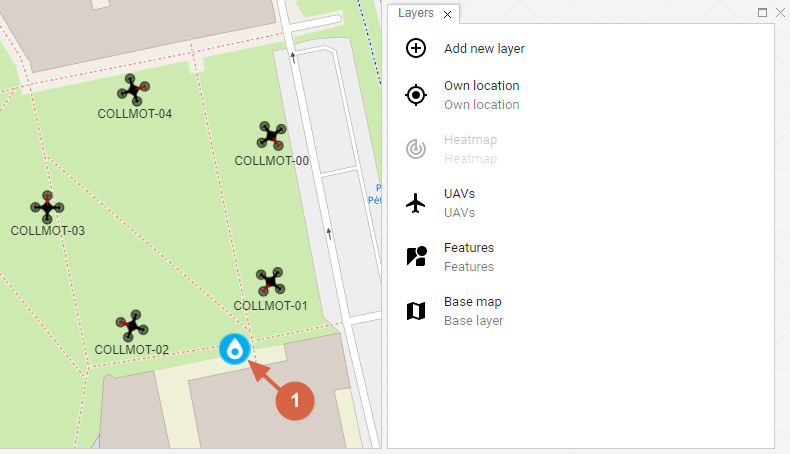
\includegraphics[width=\textwidth]{screenshots/ownlocation.png}
  \caption{A kliens állomás pozícióját mutató jelölő}
  \label{fig:ownlocation}
\end{figure}

\subsection{Billentyűkombinációkkal történő vezérlés}

Az alkalmazásban elérhető billentyűkombinációk bárhonnan működnek, amennyiben
nincsen aktív beviteli mező. A teljes lista megtekinthető a "?" szimbólum
gépelésére szolgáló billentyűkombináció lenyomásával.

A gombok olyan módon vannak megadva, hogy Windows és Linux alatt futtatva a
PlatMod ("Platform Modifier") billentyű a Control gombnak feleljen meg, míg
MacOS (OSX) rendszereken ugyanez a Command gombhoz tartozzon.

Az alapérelmezett gyorsbillentyűk kiválasztásánál fontos szempont volt az
igazodás az alapvetően elterjedt és így már megszokott kombinációkhoz. Ebből
következik például, hogy a "PlatMod + A" kombinációhoz az összes drón
kijelölése akció van hozzárendelve, míg a "PlatMod + Shift + A" lenyomásával
pedig megszüntethető a kijelölés. Hasonló elven alapul a "Ctrl + Shift + C", ami
a térképen aktuálisan a kurzor által mutatott koordináták vágólapra másolását
eredményezi.

Elérhetőek továbbá billentyűkombinációk az eszközök váltására, a térkép
megjelenésének és nézetének módosítására, valamint drónoknak kiadható parancsok
küldésére.

% TODO: \newpage

\subsection{A szűrhető és rendezhető táblák kezelése}
\label{filterable_sortable_table}

Szűrhető és rendezhető táblázaton alapul a drónok részletes állapotát mutató
panel, valamint a naplóbejegyzések megjelenítésére szolgáló lista.

Az ilyen fajta táblázatok oszlopainak fejléce fölé víve az egeret kettő gomb
válik láthatóvá. Az első az adott oszlop szerinti szűrésre, a második pedig az
adott oszlop szerinti rendezésre szolgál. A rendezés aktiválása után annak
iránya megfordítható ikonra történő ismételt kattintással.

Szűrés szempontjából három különböző fajtájú oszlop létezik.
Ezek működése illusztrálva az eseménynapló panel segítségével.
(Eredeti állapothoz lásd: \ref{fig:log}. ábra).

\begin{itemize}
  \item Előre megadott lehetőségek halmazából felvett értékek
  \begin{figure}[H]
    \center
    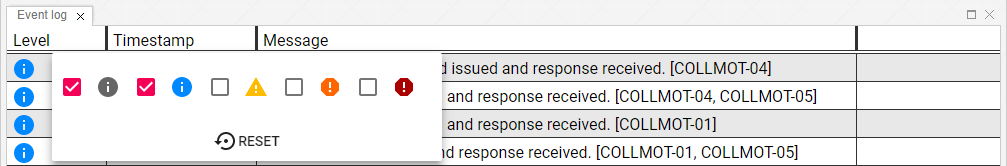
\includegraphics[width=\textwidth]{screenshots/filtered_table_list.png}
    \caption{Csak az információ típusú naplóbejegyzések megjelenítése}
    \label{fig:filtered_table_list}
  \end{figure}

  \item Intervallum típusú értékek
  \begin{figure}[H]
    \center
    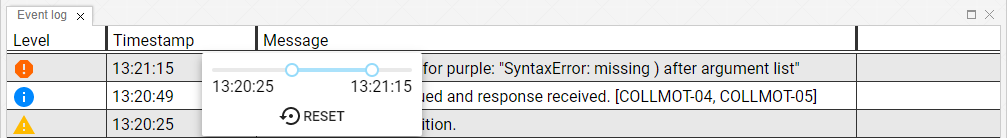
\includegraphics[width=\textwidth]{screenshots/filtered_table_range.png}
    \caption{Csak a 13:20:25 és 13:21:15 közötti naplóbejegyzések megjelenítése}
    \label{fig:filtered_table_range}
  \end{figure}

  \item Szöveg típusú értékek
  \begin{figure}[H]
    \center
    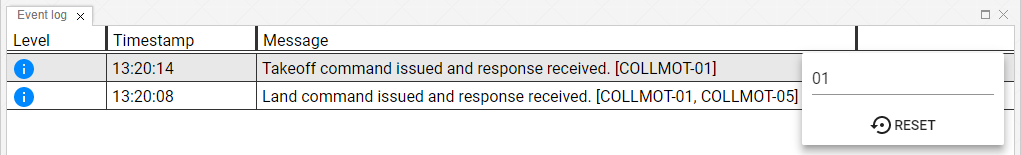
\includegraphics[width=\textwidth]{screenshots/filtered_table_text.png}
    \caption{Csak a 01-es drónnal kapcsolatos naplóbejegyzések megjelenítése}
    \label{fig:filtered_table_text}
  \end{figure}
\end{itemize}




\part{Fejlesztői dokumentáció}

\section{Funkcionális követelmények}

\subsection{Hőtérképes megjelenítés}

A drónokról érkező (numerikus) adatok megjelenítése színes hőtérkép segítségével.
A jelölő pontok méretei, a köztük lévő távolság, valamint a színskála személyre szabható (lineáris / logaritmikus, a színek határai), továbbá bekapcsolható a rácspontokhoz igazítás, ami egy négyzetrács csúcsaira illeszti a kapott értékeket.

\begin {itemize}
  \item \textit{Given} that a heatmap layer is active and is subscribed to a channel on a drone \textit{when} new data arrives from the sensor \textit{then} it is displayed on the map.
  \item \textit{Given} that there is already data, \textit{when} a new value is received, that is below the current minimum or above the current maximum, \textit{then} the color scale is adjused accordingly.
\end {itemize}


\subsection{Térkép állapotainak (pozíció, forgatás, nagyítás) tárolása és betöltése}

Egy panel, amelyen elmenthetőek, szerkeszthetőek és visszatölthetőek adott nézetek. A tárolt adatok: a középpont koordinátái, az elforgatás szöge, a nagyítás mértéke, valmint a nézet neve.

\begin {itemize}
  \item \textit{Given} that the user has moved, rotated and zoomed the map to the desired state \textit{when} the user presses the "Add a new location" button \textit{then} the actual position, rotation and zoom state is stored and the user is prompted for a name.
  \item \textit{Given} that the user has previously stored a location \textit{when} the user select that location \textit{then} the map view is moved, rotated and zoomed to match the stored data.
\end {itemize}


\subsection{Objektumok betöltése GeoJSON formátumból}

Különböző alakzatok megjelenítése a térképen, például repülési zóna vizualizálására, tereptárgyak kijelölésére.

\begin {itemize}
  \item \textit{Given} that the user has created a new layer, \textit{when} the user has selected the GeoJSON layer type, \textit{then} the application displays an input field.
  \item \textit{Given} that the input is valid GeoJSON, \textit{when} the user clicks the import button, \textit{then} the objects described in the input appear on the map.
\end {itemize}


\subsection{Parancsok kiadása drónoknak menüsorról és jobb egérgombra felugró ablakból}

Felszállás, leszállás, viszatérés illetve egyéb parancsok és üzenetek küldése drónoknak. Ha vannak kiválasztott egységek, akkor a menüsoron lévő akciók az összes jelenleg kijelölt kopterre hatással vannak, egy kopterre jobb egérgombbal kattintva pedig egy felugró ablakban válnak elérhetővé ugyanezek a lehetőségek arra az adott drónra vonatkozóan.

\begin {itemize}
  \item \textit{Given} that no drone is currently selected \textit{when} the user presses the right mouse button over a single drone, \textit{then} a popup menu appears that lets the user issue commands to that UAV.
\end {itemize}


\subsection{Állapotüzenetek (információk, figyelmeztetések, hibák) kijelzésére alkalmas panel}

Napló vezetése az alkalmazás különböző üzeneteiről, valamint ennek megjelenítése egy sorbarendezhető, szűrhető táblázatban.

\begin {itemize}
  \item \textit{Given} that an event produces a log entry, \textit{when} the message arrives, \textit{then} it is stored in the log.
  \item \textit{Given} that the log panel is active, \textit{when} the user clicks the order button on one of the column headers, \textit{then} the rows are ordered according to that column.
  \item \textit{Given} that the log panel is active, \textit{when} the user filters one of the columns, \textit{then} only those rows are displayed that match the criteria.
\end {itemize}


\subsection{Drónok színkódolása predikátumok alapján}

A drónok alapértelmezetten feketén jelennek meg, további színekhez pedig megadhatóak JavaScript függvénytörzsek, melyek paraméterül egy drón nevét kapják.
Amennyiben egy bizonyos színhez megadott feltétel, valamely azonosítót kapva paraméterként, igazra értékelődik ki, akkor az adott drón a térképen olyan színnel jelenik meg.
Például \verb|blue: 'Number(id) < 10'| esetén az 5-ös azonosítójú drón kék lesz, a 15-ös azonban nem.

\begin {itemize}
  \item \textit{Given} that there are no matching predicates, \textit{when} a drone is rendered onto the map, \textit{then} it's color is black.
  \item \textit{Given} that the user has entered a valid predicate for color A, \textit{when} the predicate evaluates to a truthy value for drone B, \textit{then} drone B is displayed in color A.
\end {itemize}


\subsection{Drónok részletes aktuális állapotát mutató panel}

Egy táblázat, amiben minden drónhoz egy-egy sor tartozik, melyben a rá vonatkozó részletes információk (akkufeszültség, aktuálisan futó algoritmus / koreográfia, stb.) láthatóak.

\begin {itemize}
  \item \textit{Given} that the information panel is active, \textit{when} the user clicks the sort button \textit{then} the rows are ordered with respect to the appropriate column.
  \item \textit{Given} that the user has selected a row with the arrow keys, \textit{when} the user presses enter \textit{then} the message dialog of the selected UAV appears.
\end {itemize}


\subsection{Kliens állomás pozíciójának megjelenítése a térképen geolokáció alapján}

Amennyiben a kliens eszköz rendelkezik geolokáció szolgáltatással, akkor a megfelelő réteg hozzáadását követően megjelenik az aktuális helyzete és iránya a térképen.
A funkció bekapcsolását követően a jelölő pozíciója és állása folyamatosan frissül az eszköz által rendelkezésre bocsátott információk alapján.

\begin {itemize}
  \item \textit{Given} that the device in use supports geolocation \textit{when} the user adds the geolocation layer, \textit{then} the marker appears.
  \item \textit{Given} that the geolocation layer has been added, \textit{when} the user moves, \textit{then} the marker moves as well.
  \item \textit{Given} that the geolocation layer has been added, \textit{when} the user turns, \textit{then} the marker turns as well.
  \item \textit{Given} that the geolocation layer has been added, \textit{when} the user deletes the geolocation layer, \textit{then} the marker disappears.
\end {itemize}


\subsection{Billentyűkombinációkkal történő vezérlés}

Az alkalmazás bizonyos funkcióinak elérése a billentyűzet segítségével, például kijelölés kezelése, parancs küldése drónoknak, dialógusablakok megnyitása.
Súgó elérése a billentyűkombinációk megtekintésére.

\begin {itemize}
  \item \textit{Given} that no input field is active, \textit{when} the user presses the "?" key, \textit{then} the available hotkeys are displayed.
  \item \textit{Given} that no input field is active, \textit{when} the user presses a hotkey, \textit{then} the desired action is performed.
\end {itemize}

\section{A szoftver architektúrája}

\subsection{Futási környezet}

A program webes technológiákon alapul, így működtethető böngészőből, illetve
böngészőtől független önálló becsomagolt állományból is.

\subsection{Felhasznált könyvtárak}

\begin{itemize}
  \item Electron: Az önlállóan futtatható állomány létrehozásához. \\
  https://electronjs.org/

  \item Redux: Az alkalmazás központi állapotának tárolásához és kezeléséhez. \\
  https://redux.js.org/

  \item Golden Layout: A dinamius, felhasználó által személyre szabható felület
  kialakítására. \\
  https://golden-layout.com/

  \item Material UI: A felhasználói felületen megjelenő elemek kinézetéhez. \\
  http://www.material-ui.com/ |  https://material-ui-next.com/

  \item OpenLayers: A térképes megjelenítéshez. \\
  https://openlayers.org/

  \item React: Minden másra? :D \\
  https://reactjs.org/

  \item ol-react: Az OpenLayers könyvtár által nyújtott funkciók React
  komponensekként való kezeléséhez. \\
  https://www.npmjs.com/package/ol-react

  \item mini-signals: Az alkalmazás komponensei közötti üzenetküldésre. \\
  https://github.com/Hypercubed/mini-signals
\end{itemize}

\subsection{A megvalósított osztályok}

\subsubsection{HeatmapLayerSettingsPresentation}
A hőtérkép réteg beállításait tartalmazó komponens.
Itt adhatóak meg az aktuális réteg úgymond "feliratkozásai", tehát, hogy melyik
eszköz melyik csatornáján érkező adatok megjelenítését végezze.
Beállítható továbbá a jelölők közötti távolság, hogy rácspontokon kerüljenek-e
elhelyezésre, vagy pedig minél közelebb a mérés helyéhez, valamint a skála
végpontjai, hogy automatikusan skálázódjon-e újabb extremális érétkek
érkezésekor, illetve hogy lineáris vagy pedig logaritmikus legyen.

\subsubsection{HeatmapVectorSource}
Az \verb|ol-react| csomag által biztosított \verb|source.Vector| osztályból
származtatott osztály, amely a hőtérképen megjelenő színes jelölők
létrehozásáért és frissítéséért felelős.
A drónokról érkező üzenetek feldolgozása és az adatok \verb|localStorage|-be
történő szinkonizálása is ebben az objektumban történik, így újratöltéskor nem
vesznek el az eddigi mérés eredményei.

\subsubsection{HeatmapLayerPresentation}
A hőtérképet megjelenítő réteg. Kirajzolja a vektor forrásból származó jelölőket
és a térkép sarkába pedig egy skálát az értékekhez.

\subsubsection{MapReferenceRequestHandler}
A központi OpenLayers térkép példány objektumhoz történő közvetlen hozzáférésre
a programban több helyen is szükség van. Ez a komponens szolgál az ilyen jellegű
igények kielégítésére oly módon, hogy feliratkozik a központi
\verb|mapReferenceRequestSignal| jelzésre, és minden ezen keresztüli üzenetben
érkező callback függvényt meghív a térkép objektum referenciájával
paraméterként, amihez oly módon fér hozzá, hogy a térkép React komponensének
leszármazottjaként a kontextus objektumából el tudja érni.

\subsubsection{MapViewManager}
A központi OpenLayers térkép példány nézeti objektumának kezelésére szolgáló
osztály. Folyamatosan tárolja az aktuális pozítiót, elfordulást és nagyítást,
valamint feliratkozik az ezekhez tartozó eseményekhez, hogy mindig frissíteni
tudja az értékeket, ha szükséges, így ezek az adatok bármikor lekérdezhetőek
belőle. Ezen felül képes a térkép nézeti paraméterének módosításaira is például
egy elmentett állapot visszatöltéséhez, vagy mondjuk adott drónhoz ugráshoz.

\subsubsection{SavedLocationEditorDialog}
Az elmentett térképállapotok szerkesztésére szolgáló dialógusablak, amelyben
szerkeszthető egy adott bejegyzés neve, középpontjának szélességi és hosszúsági
foka, elforgatási szöge és nagyítási mértéke.

\subsubsection{SavedLocationList}
Az elmentett térképállapotok felsorolására szolgáló lista, melynek első eleme
állandóan a jelenlegi állapotot tartalmazza, és arra történő kattintással az
aktuális adatok felvehetőek a listába.

\subsubsection{GeoJSONLayerSettingsPresentation}
\subsubsection{GeoJSONVectorSource}
\subsubsection{GeoJSONLayerPresentation}

\subsubsection{MapToolbar}
\subsubsection{ContextMenu}

\subsubsection{FilterableSortableTable}
\subsubsection{LogPanel}

% A naplóbejegyzéseket tartalmazó panel.

\subsubsection{OwnLocationLayerSettingsPresentation}
\subsubsection{OwnLocationVectorSource}
\subsubsection{OwnLocationLayerPresentation}

% A felhasználó geolokációjának térképen való megjelenítéséért felelős osztály.

\subsubsection{HotkeyHandler}

% A billentyűparancsok érzékeléséért és a hozzájuk rendelt feladatok végrehajtásáért felelős osztály.

\begin{figure}[H]
  \centering
    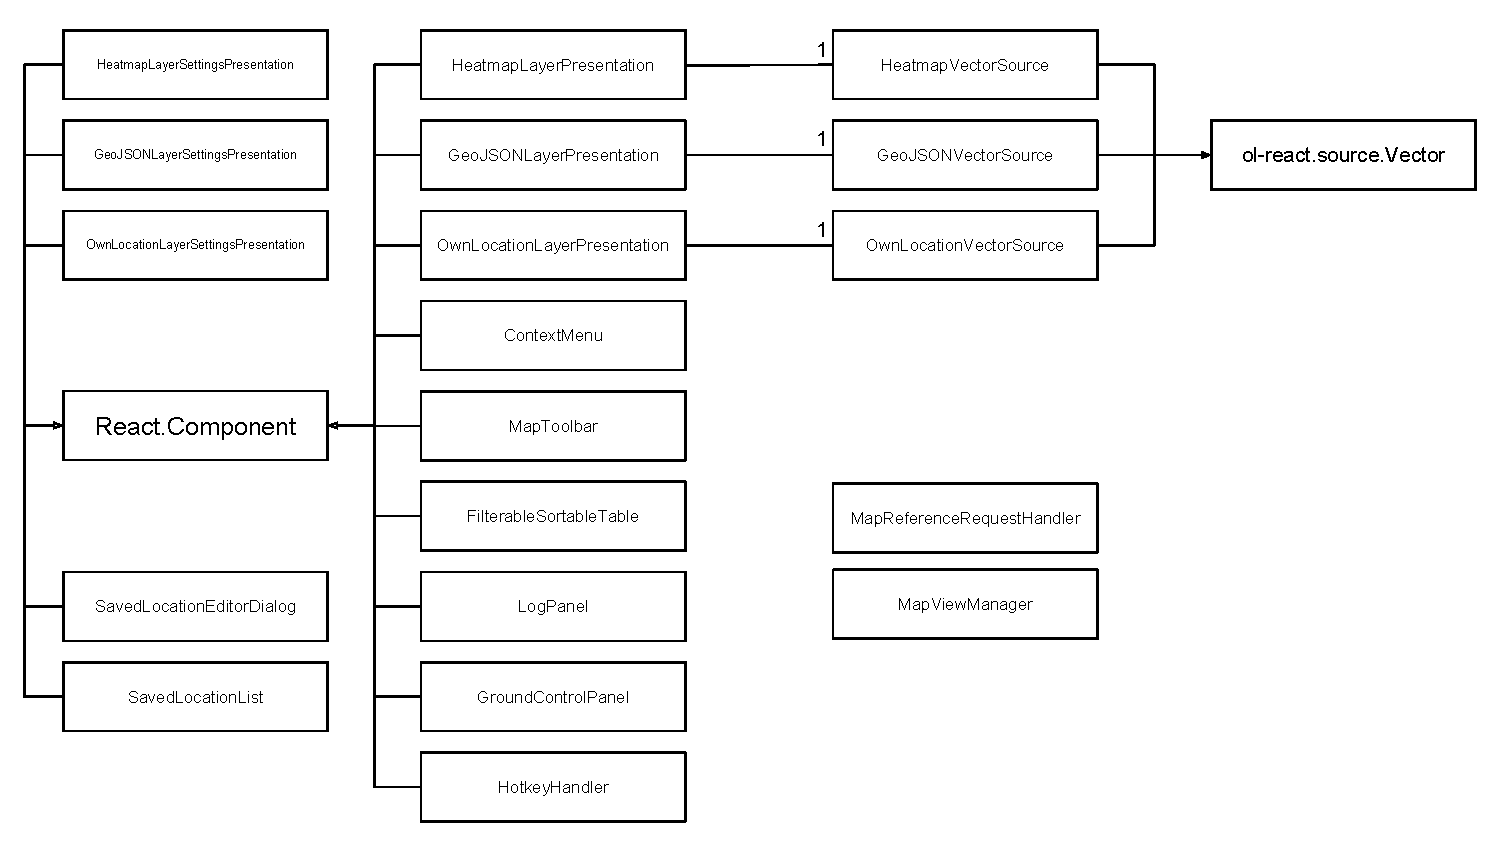
\includegraphics[width=\textwidth]{class_diagram.pdf}
  \caption{Osztálydiagram}
\end{figure}

\section{Háttér modell}

Mint az már korábban említésre került, a modell és a kontroller szerepét
egyaránt a Redux csomag tölti be. A háttérben több kisebb független modell
összekapcsolásával jön létre egy nagyobb állapot, melyeknek a módosítása
kizárólag előre megadott akciók segítségével történik, így garantálva a
konzisztenciát. Ezek közül az program általam megvalósított részeihez a
következők relevánsak:

\begin{itemize}

  \item \textbf{layers.uavs.parameters.colorPredicates}

    A drónokhoz tartozó réteg paraméterei közül a színkódolásért felelős
    predikátumok tárolása is a Redux store-ban történik. Erre egy olyan objektum
    szolgál, melynek kulcsai az elérhető színek, az ezekhez rendelt értékek
    pedig a predikátum függvények törzsei.

    \textit{Módosítására szolgáló műveletek:}

    \begin{itemize}
      \item SET\_LAYER\_PARAMETER\_BY\_ID \\
        A rétegek paramétereinek beállítására szolgáló általános akció.
        Amennyiben a koptereket megjelenítő réteg azonosítójával és a
        "colorPredicates" paraméterrel kerül meghívásra, akkor az argumentumként
        adott predikátumokat eltárolja és érvénybe lépteti.
    \end{itemize}

  \item \textbf{log}

    Az eseménynapló bejegyzéseit tartalmazó állapot. Adattípus tekintetében egy
    listaként valósul meg, amiben időrendi sorrendben szerepelnek olyan
    objektumok, melyek egy adott üzenetnek tartalmazzák az azonosítóját,
    időbélyegét, kritikussági szintjét és szövegét.

    \textit{Módosítására szolgáló műveletek:}

    \begin{itemize}
      \item ADD\_LOG\_ITEM \\
        A kapott paraméterek alapján létrehoz egy új naplóbejegyzést, amit ellát
        az aktuális időbélyeggel és hozzáadja a tárolásra szolgáló listához.

      \item DELETE\_LOG\_ITEM \\
        Törli a megadott azonosító által jelölt naplóbejegyzést.

      \item CLEAR\_LOG\_ITEMS \\
        Kiüríti a naplót, törölve ezzel az összes bejegyzést.

      \item UPDATE\_LOG\_PANEL\_VISIBILITY \\
        A naplóbejegyzések megjelenítésére szolgáló lista láthatóságának
        változásakor kezdeményezett akció. Paraméterként megkapja, hogy éppen
        megnyílt, vagy pedig bezáródott a panel.
        A bal oldali sávon a panel ikonja mellett megjelenő, olvasatlan kritikus
        üzeneteket jelző színes jelölőhöz szükséges.

    \end{itemize}

  \item \textbf{saved-locations}

    Az eltárolt pozíciók adatait (név, középpont, nagyítás, elforgatás)
    tartalmazó objektumokból álló állapot.

    \textit{Módosítására szolgáló műveletek:}

    \begin{itemize}
      \item UPDATE\_SAVED\_LOCATION \verb|(savedLocation)| \\
        Meglévő elmentett pozíció módosítása, vagy ha a paraméterként kapott
        pozíció az éppen aktuális pozíció, akkor új bejegyzés létrehozása.

      \item DELETE\_SAVED\_LOCATION (savedLocationId) \\
        Egy előzőleg elmentett pozíció törlése annak azonosítója alapján.
    \end{itemize}

\end{itemize}

\noindent Perzisztencia céljából ezen állapot bizonyos részei kerülnek adott időközönként
automatikusan mentésre a böngésző által felkínált \verb|localStorage| API
segítségével, az alkalmazás megnyitásakor pedig innen töltődnek be, így például
a beállított színek és az elmentett térkép állapotok megmaradnak az oldal
frissítése után is.


\part{Befejezés}

\paragraph{Kiegészítés:}
A projekt során a nyílt forráskódú ol-react csomag fejlesztésében is
közreműködtünk, amely az OpenLayers által nyújtott funkciók React alapú
alkalmazásokba történő integrálását segíti elő. Az elágazásunkban végzett
módosításaink egy része időközben beolvasztásra kerültek az eredeti ágba, így a
jelenleg interneten elérhető legfrissebb verzió már magában foglalja őket.

\section{Kitekintés}

A jövőre nézve a projekt továbbfejlesztésének nagyon sok iránya képzelhető el.

Ezek közül néhány példát hozva megemlíteném a más gyártótól származó drónokkal
való kommunikáció megvalósításának lehetőségét. A kereskedelmi forgalomban
elterjedtebb márkájú kopterek közül jó néhány rendelkezik nyíltan közzétett
specifikációval a rádiós kommunikációját illetően, továbbá sokszor azoknak a
drónoknak is megtalálható a visszafejtett protokolljuk, amelyek nem rendelkeznek
ilyen jellegű publikus dokumentációval.

Egy másik lehetőség azon az észrevételen alapul, hogy a mai világban már
igencsak elterjedt mobil eszközöknek köszönhetően sokaknak a zsebében lapul
webböngészővel és kellő számítási kapacitással rendelkező számítógép, ami így
tulajdonképpen már jelenlegi állapotában is alkalmas a szoftver futtatására,
viszont a szóban forgó eszköz képernyőjének méretéből és a felület
elrendezéséből adódóan nem nyújt kényelmes felhasználói élményt. Érdemes lehet
tehát létrehozni egy külön mobil verziót, amely mondjuk egyszerre csak egy panel
megjelenítését végzi. Ehhez a forráskód nagy részét újra lehetne hasznosítani a
programot alkotó React komponensek modularitásának köszönhetően. Sok kisebb
képernyőn megjelenő panelből akár összeállítható lenne egy nagyobb vezérlő
felület is, mint mondjuk egyfajta műszerfal.

Egy várhatóan hamarosan elkészülő, de a jelen szakdolgozat íródásának
időpontjában még nem elérhető funkció továbbá a drónok telepfeszültségének
jelzése a térképen, így egy leszállás után könnyebben meg lehetne találni, hogy
melyik kopterek akkumulátorait szükséges lecserélni a következő felszállás
előtt.

\section{Összefoglalás}

A szoftver tehát a bejelentőben felsorolt funkciókat megvalósítja, jelenlegi
állapotában alkalmas egy drónflotta térkép segítségével történő vizuális
kezelésére, a drónokon lévő műszerek által mért adatok megjelenítésére.

Többször is volt tesztelve valódi drónokkal, ezek közül egyik alkalomra a
2017-ben Budapesten megrendezésre kerülő FINA Vizes Világbajnokság megnyitójának
főpróbáján került sor. A mellékelt képek mutatják a drónok elhelyezkedését a
rakparton (\ref{fig:fina_launch}. ábra), és az ezzel a képpel közel egy időben készült
képernyőfelvételt a szoftver akkor aktuális állapotáról
(\ref{fig:fina_launch_screen}. ábra), melyen megjelennek az elérhető kopterek.

\begin{figure}[H]
  \includegraphics[width=\textwidth]{fina_launch.jpg}
  \caption{Egy Duna-parti felszállás előtt}
  \label{fig:fina_launch}
\end{figure}

\begin{figure}[H]
  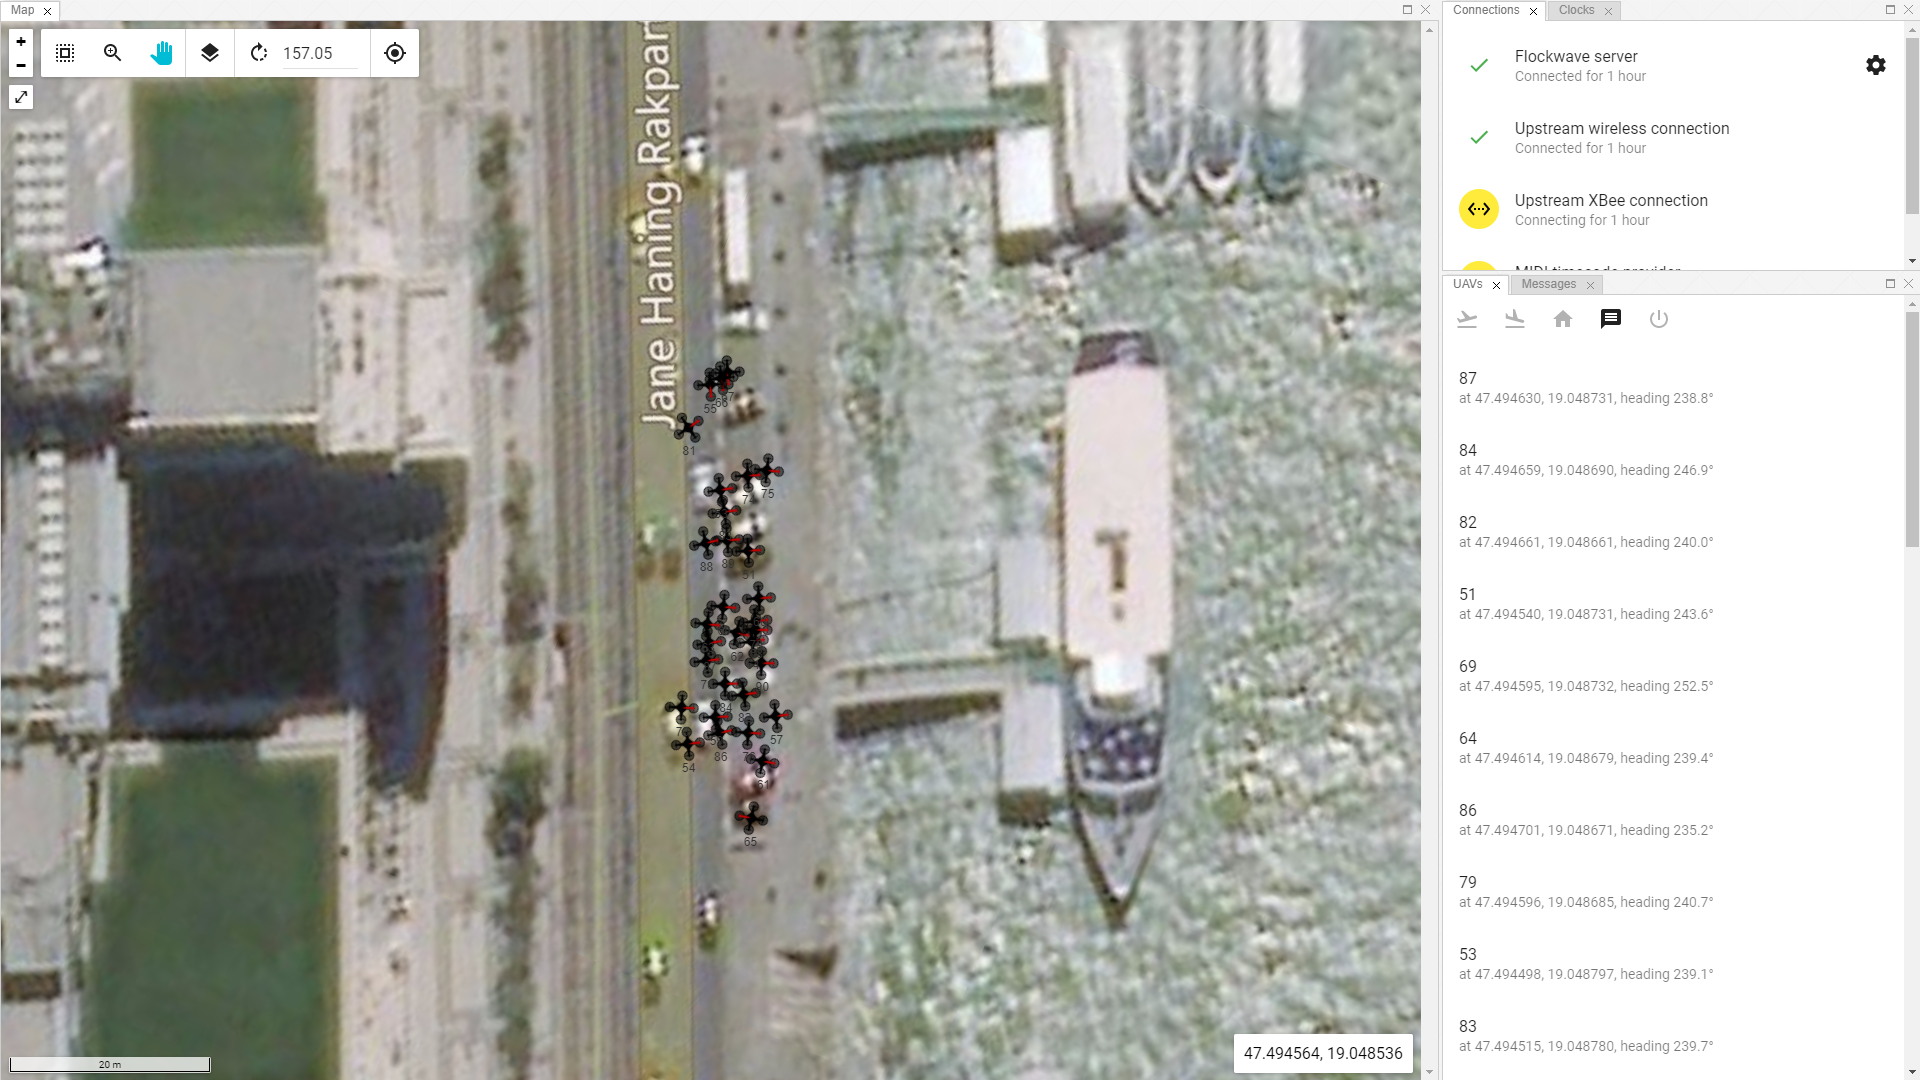
\includegraphics[width=\textwidth]{fina_launch_screen.png}
  \caption{Egy Duna-parti felszállás előtt (képernyőkép)}
  \label{fig:fina_launch_screen}
\end{figure}

A szoftver fejlesztése továbbra is folyamatosan zajlik, állandóan új és új
funkciókkal bővül és időről időre tesztelésre is kerül.


\end{document}
